\chapter{Cálculo no lineal mediante elementos finitos}
\label{cap3}


\section{Objetivos de la práctica}
\label{sec:objetivos}

En esta práctica se desarrolla la simulación mediante elementos finitos del comportamiento del tejido biológico blando, empleando modelos hiperelásticos no lineales y grandes deformaciones, mediante el programa FEBiO \cite{FEBiO}.
En particular se desarrollan los siguientes modelos:
\begin{enumerate}
	\item
	En primer lugar se desarrolla la solución analítica mediante modelos de material hiperelástico incompresible, que será empleada posteriormente para comparar con las soluciones numéricas (sección \ref{sec:anal}).
	\item
	Se simula de la deformación \emph{homogénea} en un punto del tejido, mediante un modelo con un único elemento, sometido a tracción uniaxial sin confinar (sección \ref {sec:homog}).
	\item
	Se simula de la deformación de una arteria comprimida en una sección con un modelo discretizado con varios elementos aprovechando diferentes simetrías.  (sección \ref {sec:arteria}).
	\item
	Se proponen algunas tareas a llevar a cabo por los estudiantes para evaluar el aprovechamiento de la práctica (sección \ref{sec:tareas}).
\end{enumerate}


\section{Base teórica y solución analítica}
\label{sec:anal}

%\subsection{General equations}
\subsection{Ecuaciones generales}

%Consider a hyperelastic material defined with the energy density function $W$ per unit reference volume, the PK stress is obtained as
Se considera un material hiperelástico definido, en la configuración de referencia, mediante la función de densidad de energía por unidad de volumen,
\begin{equation}
  \bm{S} = 2\frac{\partial W}{\partial\bm{C}}\,,
\end{equation}
%in terms of the Cauchy-Green tensor
siendo 
$\bm{C}=\bm{F}^\text{T}\cdot\bm{F}$ 
el tensor de deformación de Cauchy-Green
%and $\bm{S} the second Piola-Kirchhoff stress tensor (PK).
y $\bm{S}$ el tensor de tensiones segundo de Piola-Kirchhoff (PK). 
%We assume an isotropic material with principal stretches
Suponemos un material isótropo, con deformación caracterizada por las extensiones principales 
$(\lambda_1,\lambda_2,\lambda_3)$, 
%using coordinates along these local principal directions the component matrices of the deformation gradient and the Cauchy-Green tensor are diagonal
por lo que tomando coordenadas según estas direcciones principales las matrices de componentes son
\begin{equation}
  [\bm{F}]=\begin{pmatrix}
  \lambda_1 & 0 & 0 \\ 0 & \lambda_2 & 0 \\ 0 & 0 & \lambda_3
  \end{pmatrix}
  \,;\quad
  [\bm{C}]
  =\begin{pmatrix}
  C_1 & 0 & 0 \\ 0 & C_2 & 0 \\ 0 & 0 & C_3
  \end{pmatrix}
  =\begin{pmatrix}
  \lambda_1^2 & 0 & 0 \\ 0 & \lambda_2^2 & 0 \\ 0 & 0 & \lambda_3^2
  \end{pmatrix}
  \,.
  \label{eq:FC}
\end{equation}
%The PK stress can be also expressed along the same coordinates,
La tensión PK resulta también alineada con las mismas direcciones principales,
\begin{equation}
  [\bm{S}]=2\begin{pmatrix}
  {\partial W}/{\partial C_1} & 0 & 0 \\ 
  0 & {\partial W}/{\partial C_2} & 0 \\
  0 & 0 & {\partial W}/{\partial C_3}
  \end{pmatrix}
  \,.
  \label{eq:S}
\end{equation}
%Taking into account the previous expression for 
Teniendo en cuenta la expresión anterior de 
$\bm{C}$ 
%and the chain rule we obtain
y la regla de la cadena resulta:
\begin{equation}
  S_i = 2 \frac{\partial W}{\partial \lambda_i}\frac{\partial\lambda_i}{\partial
  C_i} = \frac{\partial W}{\partial \lambda_i}\frac{1}{\lambda_i}
%  \quad\text{(no  sum in index $i$)}
  \quad\text{(sin sumatorio en índice $i$)}
  \,.
  \label{eq:Si}
\end{equation}
%The Cauchy stress is also aligned with the same principal directions,
La tensión de Cauchy está alineada también con las mismas direcciones principales, al ser su relación con el tensor de PK la siguiente
\begin{equation}
  \bm{\sigma} = J^{-1}\bm{F}\cdot\bm{S}\cdot\bm{F}^\text{T}
  \,,
\end{equation}
%hence the principal Cauchy stresses (true stresses) results
por lo que las tensiones principales de Cauchy (verdaderas) resultan
\begin{equation}
  \sigma_i = J^{-1} \lambda_i\frac{\partial W}{\partial\lambda_i}
  \,.
  \label{eq:sigmai}
\end{equation}

%Consider now the incompressible case. The constraint for constant volume is expressed as
Consideramos ahora el caso incompresible. Se introduce la restricción de volumen constante
\begin{equation}
  J=\lambda_1\lambda_2\lambda_3 = 1
  \,.
  \label{eq:incomp}
\end{equation}
%This constraint causes an indetermination in the expressions \eqref{eq:sigmai} for the stresses.
%In particular the pressure $p$ may not be defined from the constitutive equations of the material.
%In simple cases, $p$ may be calculated with the boundary conditions and introduced in the equation for stresses:
Esta restricción origina una indeterminación en las expresiones \eqref{eq:sigmai} de las tensiones, en función de una presión $p$, a priori desconocida
\begin{equation}
  \sigma_i = \lambda_i\frac{\partial W}{\partial\lambda_i} -p
  \,.
  \label{eq:sigmai-incomp}
\end{equation}
El valor de $p$ no se puede obtener mediante las ecuaciones constitutivas del material y  deberá ser calculada en cada caso a partir de las condiciones de contorno.

%Assume now the uniaxial stress case, for which we shall take the principal stretch $\lambda_1$ along the loaded direction.
%The stretches along the two transverse directions will be equal $\lambda_2=\lambda_3$, and from the incompressibility condition \eqref{eq:incomp} we arrive to $\lambda_1 = 1/\lambda_2^2$.
%On the other hand, in the transverse directions the stress is zero, allowing the determination of $p$:
Suponemos ahora el caso de tensión uniaxial, según esta dirección tomaremos la extensión principal $\lambda_1$. Las deformaciones en las dos direcciones laterales serán iguales $\lambda_2=\lambda_3$, y de la condición de incompresibilidad \eqref{eq:incomp} se deduce $\lambda_1 = 1/\lambda_2^2$. 
Por otra parte, en las direcciones laterales la tensión es nula, permitiendo estas condiciones de contorno la determinación de $p$:
\begin{equation}
  \sigma_2 = \sigma_3 = 0 
  \quad\Rightarrow\quad 
  p=\lambda_2\frac{\partial W}{\partial\lambda_2}
  \,,
\end{equation}
%and substituting in
y sustituyendo en 
\eqref{eq:sigmai-incomp} 
%the following relationship between stress and stretch is obtained:
resulta la relación entre la tensión y el alargamiento:
\begin{equation}
	\mathbox{
  \sigma_1 = \lambda_1\frac{\partial W}{\partial\lambda_1} - 
  \lambda_1^{-1/2}\frac{\partial W}{\partial\lambda_2}
  \,.
  }
  \label{eq:tuni}
\end{equation}
%This general expression may then be applied to particular cases of hyperelastic materials with specific functions for strain energy density $W$.
Esta expresión general se puede aplicar a casos particulares de materiales hiperelásticos con funciones específicas de densidad de energía $W(\lambda_{i})$.

%\subsection{Neohookean material}
\subsection{Material Neohookeano}
%Let us consider an incompressible Neohookean material, defined with the energy density function
Consideramos un material Neohookeano incompresible, definido por la función de energía
\begin{equation}
  W = \frac{\mu}{2}\left(I_1-3\right)
  \,,
  \label{eq:neoh}
\end{equation}
%where
donde el invariante principal 1 se expresa en función de las extensiones principales como
$I_1=\lambda_1^2+\lambda_2^2+\lambda_3^3$.

En FEBiO \cite{febio-tmanual} el material Neohookeano se obtiene como un caso particular del material de Mooney-Rivlin,
\begin{equation}
	\bar W = c_{1} (\bar I_{1}-3) + c_{2} (\bar I_{1}-3)
	\,,
\end{equation}
tomando $c_{1}=\mu/2$ y $c_{2}=0$.
%Applying \eqref{eq:tuni} the stress-stretch expression is obtained directly:
Aplicando \eqref{eq:tuni} se obtiene directamente la expresión tensión--alargamiento:
\begin{equation}
	\mathbox{
  \sigma = \mu(\lambda^2-\lambda^{-1})
  \,,
  }
  \label{eq:neoh-tuniax}
\end{equation}
%where we have called
donde hemos denominado 
$\lambda=\lambda_1$ 
%and
y 
$\sigma=\sigma_1$.

Como ejemplo se muestra el caso $\mu=2 c_{1}=80$ kPa en la figura \ref{fig:neoh-anal}.
\begin{figure}[!htp]
\centering
\includegraphics[width=0.6\textwidth]{figuras_3/neoh-anal.eps}
\caption{Solución analítica uniaxial del modelo Neohookeano ($\mu=80$ kPa)}
\label{fig:neoh-anal}
\end{figure}

%\subsection{Ogden material}
\subsection{Material de Ogden}
\label{sec:ogden}

%The Ogden incompressible material is defined by the following energy density function
El material incompresible de Ogden se define por la siguiente función de densidad de energía
\begin{equation}
	W = \sum_{i=1}^{N} \frac{C_{i}}{a_{i}}
	\big(\lambda_{1}^{a_{i}}+\lambda_{2}^{a_{i}}+\lambda_{3}^{a_{i}}-3\big)
	\label{eq:ogd}
\end{equation}
%with the volumetric term $U(J)=\frac{1}{2}k(\ln J)^{2}$.
%In \cite{febio} the function is expressed with a slightly different definition of the terms,
En FEBiO \cite{febio-tmanual} la función se expresa con una definición ligeramente distinta de los parámetros,
\begin{equation}
	W = \sum_{i=1}^{N} \frac{c_{i}}{m_{i}^{2}}
	\big(\lambda_{1}^{m_{i}}+\lambda_{2}^{m_{i}}+\lambda_{3}^{m_{i}}-3\big)
	\label{eq:ogd-feb}
\end{equation}
%The equivalence between both is given by 
La equivalencia entre ambos viene dada por
$C_{i}=c_{i}/m_{i}, a_{i}=m_{i}$.

%Applying \eqref{eq:tuni} the stress-stretch expression is obtained directly:
Desarrollando la expresión \eqref{eq:tuni} se obtiene directamente la expresión tensión--alargamiento:
\begin{equation}
  \sigma = \sum_{i=1}^{N} C_{i}\big( \lambda^{a_{i}}-\lambda^{-a_{i}/2}\big)
  \,,
  \label{eq:ogdenh-tuniax}
\end{equation}
%We consider here for simplicity a model with only one term $(N=1)$.
%In this case the stress-strech response will be
Consideramos aquí por simplicidad un modelo con un único término $(N=1)$.
En este caso, la relación tensión--alargamiento será
\begin{equation}
	\mathbox{
  \sigma = C_{1}\big( \lambda^{a_{1}}-\lambda^{-a_{1}/2}\big)
  \,.
  }
  \label{eq:ogdenh-tuniax1}
\end{equation}

Como ejemplo se muestra el caso ($N=1$, $c_{1}=6.58$ kPa, $a_{1}=m_{1}=6.83$) en la figura \ref{fig:ogden-anal}.
\begin{figure}[!htp]
\centering
\includegraphics[width=0.6\textwidth]{figuras_3/ogden-anal.eps}
\caption{Solución analítica uniaxial del modelo de Ogden ($N=1$, $c_{1}=6.58$ kPa, $m_{1}=6.83$).}
\label{fig:ogden-anal}
\end{figure}


\section{Extensión uniaxial homogénea con FEBiO}
\label{sec:homog}

\subsection{Geometría y malla}
\label{sec_modelo-h}

Desarrollamos en primer lugar un modelo sencillo, con un único elemento, y deformado de manera homogénea mediante la extensión uniaxial en dirección perpendicular a una de sus caras, sin confinamiento alguno en las caras laterales.
Naturalmente esto obliga a que la tensión sea también uniforme a lo largo del modelo.
Este caso servirá para verificar la la ecuación constitutiva del material.
Asimismo permite una introducción sencilla a la elaboración y cálculo de un modelo no lineal con FEBiO.

La geometría será un hexaedro con dimensiones $1\times 1\times 1$ mm$^{3}$, para el que supondremos además condiciones de simetría en los planos dorsales normales a $x$, $y$ y $z$.
(Por tanto el cuerpo físico real al que corresponde el modelo tendría dimensiones $2\times 2\times 2$ mm$^{3}$.)
En el plano superior $z=1$ aplicaremos un desplazamiento impuesto de valor $u_{z}=1.5$, que equivale a un estiramiento en esta dirección de valor $\lambda=(1+1.5)/1=2.5$.
El comportamiento del material lo supondremos según los modelos Neohookeano y de Ogden descritos en la sección anterior.

En primer lugar abrimos el programa \emph{Febio Studio} y comenzamos con un nuevo modelo, obteniendo la ventana de la figura \ref{fig:pre-00}.
A continuación en la ventana del módulo \emph{build} (lado derecho) crearemos un hexaedro, centrado en $(0,0,0)$ y con dimensiones $(1,1,1)$, fig. \ref{fig:pre-01}.
\begin{figure}[!ht]
\centering
\begin{subfigure}[b]{0.48\textwidth}
\includegraphics[width=\linewidth]{figuras_3/scr-pre-00.png}
\caption{Ventana de apertura de Preview}
\label{fig:pre-00}
\end{subfigure}
\begin{subfigure}[b]{0.48\textwidth}
\includegraphics[width=\linewidth]{figuras_3/scr-pre-01m.png}
\caption{Crear geometría de hexaedro}
\label{fig:pre-01}
\end{subfigure}
\caption{Apertura de Preview y creación de geometría}
\label{fig:pre-00-01}
\end{figure}
A continuación definimos la malla sobre esta geometría, en la pestaña \emph{Mesh}, empleando un único elemento ($N_{x}=N_{y}=N_{z}=1$, fig. \ref{fig:pre-02}); al activar con el botón \fbox{\emph{Apply}} se obtiene la imagen de la fig. \ref{fig:pre-02}, con losparámetros de la malla.
\begin{figure}[!htp]
\centering
\begin{subfigure}[b]{0.48\textwidth}
\centering
\includegraphics[width=0.5\linewidth]{figuras_3/scr-pre-02m.png}
\caption{Parámetros de la malla (1 elemento)}
\label{fig:pre-02}
\end{subfigure}
\begin{subfigure}[b]{0.48\textwidth}
\centering
\includegraphics[width=0.5\linewidth]{figuras_3/scr-pre-03.png}
\caption{Malla creada}
\label{fig:pre-02}
\end{subfigure}
\caption{Creación de la malla}
\label{fig:pre-02-03}
\end{figure}

\subsection{Material (Neohookeano) y condiciones de contorno}

El próximo paso es definir el material; para ello se activa el icono en la barra superior para seleccionar partes (fig. \ref{fig:pre-04}), la marcamos con el ratón, y en el módulo \emph{Model} (a la izquierda) con el botón derecho se activa \emph{add material} apareciendo una ventana para seleccionar el tipo de material, donde escogeremos \emph{elastic uncoupled} y \emph{Mooney-Rivlin} (fig. \ref{fig:pre-04}).
En los recuadros que aparecen especificamos los parámetros del material, $c_{1}=40$, $c_{2}=0$, y un módulo volumétrico suficientemente alto para garantizar la incompresibilidad $k=40000$ (fig. \ref{fig:pre-05}).
La densidad del material es irrelevante en este caso, al ser un cálculo estático, por lo que no se modifica el valor que viene por defecto ($\rho=1$).
\begin{figure}[!htpb]
\centering
\begin{subfigure}[b]{0.48\textwidth}
\includegraphics[width=\textwidth]{figuras_3/scr-pre-04m.png}
\caption{Selección del tipo de material}
\label{fig:pre-04}
\end{subfigure}
\begin{subfigure}[b]{0.48\textwidth}
\includegraphics[width=\textwidth]{figuras_3/scr-pre-05m.png}
\caption{Parámetros del material Neohookeano}
\label{fig:pre-05}
\end{subfigure}
\caption{Definición del material}
\label{fig:pre-04-05}
\end{figure}

El siguiente paso es definir las condiciones de contorno, en el módulo \emph{Model} (a la izquierda), empleando el botón derecho del ratón, sobre \emph{Boundary conditions} $\to$  \emph{Add boundary condition}.
En primer lugar definimos una condición de tipo \emph{Fixed displacement} (fig. \ref{fig:pre-06}); se activa el icono de seleccionar las caras y se escoge la cara posterior según el eje $x$, definiendo la condición como fijado \emph{X-displacement} (fig. \ref{fig:pre-07}).
Para orientarse con los ejes debe indicarse que los colores son: \textcolor{red}{\textbf rojo = $x$}, \textcolor{green}{\textbf verde = $y$}, \textcolor{blue}{\textbf azul = $z$}.
La cara correspondiente (en este caso \emph{Surface4}) debe aparecer en el recuadro inferior.
Si se comete un error en la selección puede corregirse esta con los botones al lado de este recuadro, remarcados en la figura.
\begin{figure}[!htp]
\centering
\begin{subfigure}[b]{0.48\textwidth}
\includegraphics[width=\textwidth]{figuras_3/scr-pre-06m.png}
\caption{Establecer desplazamiento fijo}
\label{fig:pre-06}
\end{subfigure}
\begin{subfigure}[b]{0.48\textwidth}
\includegraphics[width=\textwidth]{figuras_3/scr-pre-07m.png}
\caption{Condición $u_{x}=0$ en la cara $x=0$}
\label{fig:pre-07}
\end{subfigure}
\caption{Establecer condiciones de contorno}
\label{fig:pre-06-07}
\end{figure}
A continuación se establecen de igual manera, seleccionando las caras correspondientes, las condiciones de contorno de desplazamiento nulo en los otros dos planos posteriores normales a los ejes $y$ (fig. \ref{fig:pre-08}) y $z$ (fig. \ref{fig:pre-09}).
\begin{figure}[!htp]
\centering
\begin{subfigure}[b]{0.48\textwidth}
\includegraphics[width=\textwidth]{figuras_3/scr-pre-08m.png}
\caption{Condición $u_{y}=0$ en la cara dorsal $y$}
\label{fig:pre-08}
\end{subfigure}
\begin{subfigure}[b]{0.48\textwidth}
\includegraphics[width=\textwidth]{figuras_3/scr-pre-09m.png}
\caption{Condición $u_{z}=0$ en la cara dorsal $z$}
\label{fig:pre-09}
\end{subfigure}
\caption{Condiciones de contorno de desplazamiento nulo en los otros dos planos}
\label{fig:pre-08-09}
\end{figure}

Por último se define una condición de contorno en la superficie del plano superior $z=1$ de desplazamiento impuesto, seleccionando en el menú la opción \emph{Prescribed displacement} (fig. \ref{fig:pre-10}) para la cara del plano superior y definiendo el valor del desplazamiento $u_{z}=1.5$ (fig. \ref{fig:pre-11}).
\begin{figure}[!htp]
\centering
\begin{subfigure}[b]{0.48\textwidth}
\centering
\includegraphics[width=0.5\textwidth]{figuras_3/scr-pre-10.png}
\caption{Selección para desplazamiento impuesto}
\label{fig:pre-10}
\end{subfigure}
\begin{subfigure}[b]{0.48\textwidth}
\includegraphics[width=\textwidth]{figuras_3/scr-pre-11m.png}
\caption{Definición de $u_{z}=1.5$ en la cara $z=1$}
\label{fig:pre-11}
\end{subfigure}
\caption{Condiciones de contorno de desplazamiento impuesto}
\label{fig:pre-10-11}
\end{figure}

\subsection{Definición y ejecución del caso de cálculo}

Se necesita definir ahora el caso  (\emph{Step}) de cálculo, seleccionando en el menú \emph{Step} $\to$ \emph{Add step}, del tipo \emph{Structural mechanics} (fig. \ref{fig:pre-12}).
\begin{figure}[!htp]
\centering
\begin{subfigure}[b]{0.48\textwidth}
\centering
\includegraphics[width=\textwidth]{figuras_3/scr-pre-12.png}
\caption{\emph{Add step} de tipo \emph{Structural mechanics}}
\label{fig:pre-12}
\end{subfigure}
\begin{subfigure}[b]{0.48\textwidth}
\includegraphics[width=\textwidth]{figuras_3/scr-pre-13m.png}
\caption{Parámetros: $T_\text{fin}=15\times 0.1=1.5$}
\label{fig:pre-13}
\end{subfigure}
\caption{Definición del \emph{Step} de análisis}
\label{fig:pre-12-13}
\end{figure}

Definimos un número de pasos de 15 y un incremento de tiempo $\Delta t=0.1$, de forma que el tiempo final de cálculo será $T_\text{fin}=15\times 0.1=1.5$. 
Creamos una curva modificada de aplicación de la carga mediante el botón de creación/edición de curvas en el icono a la derecha de la barra superior en la fig. \ref{fig:pre-13}, y lo asignamos al desplazamiento impuesto.
Esta curva la modificamos de forma que el tiempo de aplicación sea $1.5$, cambiando el valor por defecto de $1.0$; para ello se redefine el punto como $(1.5, 1.0)$ (fig. \ref{fig:pre-14}).
Por último, se guarda el fichero (\texttt{.fsm}) de Preview, y se exporta el fichero de cálculo (\texttt{.feb}) para FEBiO (fig. \ref{fig:pre-15}).
\begin{figure}[!htp]
\centering
\begin{subfigure}[b]{0.48\textwidth}
\centering
\includegraphics[width=0.8\textwidth]{figuras_3/scr-pre-14.png}
\caption{Definición de la curva de aplicación}
\label{fig:pre-14}
\end{subfigure}
\begin{subfigure}[b]{0.48\textwidth}
\centering
\includegraphics[width=0.7\textwidth]{figuras_3/scr-pre-15.png}
\caption{Exportar al fichero de FEBiO}
\label{fig:pre-15}
\end{subfigure}
\caption{Curva de aplicación y exportación del fichero de cálculo}
\label{fig:pre-14-15}
\end{figure}

Una vez exportado ejecuta el programa FEBiO. %(\texttt{febio2.exe}) sobre el fichero exportado antes (en este caso se denomina \texttt{h-neoh.feb}), desde una ventana del intérprete de mandatos (fig. \ref{fig:feb-01}).
%Para ello habrá sido necesario situarse previamente (mandato \emph{chdir}) en el directorio donde se tiene dicho fichero de datos \texttt{.feb}.
Si todo es correcto se obtiene al final un mensaje de terminación normal como la fig. \ref{fig:feb-02}.
El cálculo produce un fichero para postproceso del tipo \texttt{.xplt} en el mismo directorio.
\begin{figure}[!htp]
\centering
\begin{subfigure}[b]{0.48\textwidth}
\centering
\includegraphics[width=\textwidth]{figuras_3/scr-feb-01.png}
\caption{Mandato de ejecución de FEBiO}
\label{fig:feb-01}
\end{subfigure}
\begin{subfigure}[b]{0.48\textwidth}
\centering
\includegraphics[width=\textwidth]{figuras_3/scr-feb-02.png}
\caption{Final correcto del cálculo}
\label{fig:feb-02}
\end{subfigure}
\caption{Cálculo con FEBiO}
\label{fig:feb-01-02}
\end{figure}

\subsection{Postproceso con Postview}

Abrimos el fichero \texttt{.xplt} en el programa \emph{Postview} de la Suite \emph{FEBio Studio} y la primera vista que se obtiene es desde el punto de vista superior $z^{+}$, fig. \ref{fig:post-01}.
Se gira con el ratón para obtener la orientación 3D deseada, y se fija la escala de forma que abarque tanto la configuración inicial (fig. \ref{fig:post-02}) como la final (fig. \ref{fig:post-03}).
Con esta escala fijada se puede obtener una animación del proceso con los iconos de la barra superior a la derecha.
\begin{figure}[!htp]
\centering
\includegraphics[width=0.5\textwidth]{figuras_3/scr-post-01.png}
\caption{Abrir fichero \texttt{.xplt} en programa \emph{Postview}}
\label{fig:post-01}
\end{figure}

\begin{figure}[!htp]
\centering
\begin{subfigure}[b]{0.48\textwidth}
\centering
\includegraphics[width=\textwidth]{figuras_3/scr-post-02.png}
\caption{Vista del modelo en $t=0$}
\label{fig:post-02}
\end{subfigure}
\begin{subfigure}[b]{0.48\textwidth}
\centering
\includegraphics[width=\textwidth]{figuras_3/scr-post-03.png}
\caption{Vista del modelo en $t=T_\text{fin}$}
\label{fig:post-03}
\end{subfigure}
\caption{Fijar escala y perspectiva}
\label{fig:post-02-03}
\end{figure}

Sin embargo resulta más representativo obtener un mapa de colores con las variables significativas del problema, en este caso la tensión $\sigma_{zz}$, que se define como se indica en la fig. \ref{fig:post-04-05}.
\begin{figure}[!htp]
\centering
\begin{subfigure}[b]{0.48\textwidth}
\centering
\includegraphics[width=\textwidth]{figuras_3/scr-post-04.png}
\caption{Seleccionar variable $\sigma_{zz}$}
\label{fig:post-04}
\end{subfigure}
\begin{subfigure}[b]{0.48\textwidth}
\centering
\includegraphics[width=\textwidth]{figuras_3/scr-post-05.png}
\caption{Mapa coloreado de $\sigma_{zz}$ en instante dado}
\label{fig:post-05}
\end{subfigure}
\caption{Definir variable a representar, $\sigma_{zz}$}
\label{fig:post-04-05}
\end{figure}
Se pueden obtener instantáneas para la animación mediante el menú \emph{Record}, o también se puede crear un fichero de vídeo, bien directamente con el menú \emph{Record} o mediante la composición de los fotogramas individuales.

Adicionalmente podemos obtener la curva de historia (evolución) de cualquier variable en cualquier entidad (nodo, cara, elemento).
En este caso obtenemos la historia de $\sigma_{zz}$ en el único elemento del problema, fig. \ref{fig:post-06-07}.
\begin{figure}[!htp]
\centering
\begin{subfigure}[b]{0.48\textwidth}
\centering
\includegraphics[width=\textwidth]{figuras_3/scr-post-06.png}
\caption{Crear curva para historia en elemento}
\label{fig:post-06}
\end{subfigure}
\begin{subfigure}[b]{0.48\textwidth}
\centering
\includegraphics[width=\textwidth]{figuras_3/scr-post-07m.png}
\caption{Historia de $\sigma_{zz}$ y valor numérico}
\label{fig:post-07}
\end{subfigure}
\caption{Obtener curva de historia $\sigma_{zz} / t$}
\label{fig:post-06-07}
\end{figure}
Por otra parte los valores numéricos para esta curva se pueden obtener en un fichero de texto, mediante el icono de salvar que se muestra en la fig. \ref{fig:post-07}.
El fichero se puede abrir con un editor de texto simple como \emph{Notepad++} (fig. \ref{fig:post-08}).
Estos resultados se pueden luego procesar junto a otros resultados o dibujar mediante algún programa especial para dibujo de curvas, fig. \ref{fig:post-09}, comparando el resultado numérico de EF con la solución analítica para este caso obtenida en la sección \ref{sec:anal}, ecuación \eqref{eq:neoh-tuniax}.
\begin{figure}[!htbp]
\centering
\begin{subfigure}[b]{0.41\textwidth}
\centering
\includegraphics[width=\textwidth]{figuras_3/notepad-szz.png}
\caption{\emph{Notepad++} con historia de $\sigma_{zz}(t)$}
\label{fig:post-08}
\end{subfigure}
\begin{subfigure}[b]{0.56\textwidth}
\centering
\includegraphics[width=\textwidth]{figuras_3/hneoh_feb.eps}
\caption{Gráfico con soluciones analítica y numérica}
\label{fig:post-09}
\end{subfigure}
\caption{Inspección y gráficos para historia $\sigma_{zz}(t)$, visualizada externamente}
\label{fig:post-08-09}
\end{figure}
Se comprueba que la coincidencia con la solución analítica es excelente.
Asimismo se puede observar que en este caso Neohookeano la no linealidad del material es moderada.

\subsection{Caso con material de Ogden}

Se desarrolla ahora un caso similar, de extensión no confinada homogénea, en esta ocasión con material de Ogden, según se ha definido en la sección \ref{sec:ogden}.
Las propiedades son las ya definidas en la sección citada.

No es necesario repetir todos los pasos anteriores para la creación del modelo, de hecho se puede aprovechar el modelo creado antes haciendo una copia del fichero \texttt{.fsm} que modificaremos posteriormente.
La modificación principal es desasignar el material Neohookeano anterior y crear un nuevo material del tipo Ogden y con las características citadas (fig. \ref{fig:01-mat-ogden}).
El único cambio adicional que haremos es definir incrementos de tiempo ligeramente más pequeños para facilitar la convergencia, que en este caso requiere más esfuerzo, ya que como veremos el carácter no lineal del material es mayor.
Para ello se toman 20 incrementos de valor $\Delta t=0.075$, sobre el mismo tiempo total $T_\text{fin}=20\times 0.075=1.5$, y con la misma curva de aplicación entre $(0,0)$ y $(1.5,1.0)$ que antes (fig. \ref{fig:02-step-ogden}).

\begin{figure}[!htp]
\centering
\begin{subfigure}[b]{0.48\textwidth}
\centering
\includegraphics[width=\textwidth]{figuras_3/01-mat-ogden.png}
\caption{Definición del material de Ogden}
\label{fig:01-mat-ogden}
\end{subfigure}
\begin{subfigure}[b]{0.48\textwidth}
\centering
\includegraphics[width=\textwidth]{figuras_3/02-step-ogden.png}
\caption{\emph{Step} para cálculo}
\label{fig:02-step-ogden}
\end{subfigure}
\caption{Definición de modelo homogéneo con material de Ogden}
\label{fig:pre-hogden}
\end{figure}

Una vez guardado el fichero y procedido a su cálculo y su posterior visualización con \emph{Postview}, se puede obtener ahora la historia temporal en FEBiO (fig \ref{fig:01-thist-ogden-szz}).
Guardando los valores numéricos en un fichero de texto, la solución numérica de FEBiO puede compararse con la solución analítica expresada en la ecuación \eqref{eq:ogdenh-tuniax1} (fig \ref{fig:hogden_feb}), obteniéndose como antes una coincidencia casi exacta.
En este caso sí se observa un efecto no lineal muy marcado, característico de muchos tejidos blandos con fibras.

\begin{figure}[!htp]
\centering
\begin{subfigure}[b]{0.43\textwidth}
\centering
\includegraphics[width=\textwidth]{figuras_3/01-thist-ogden-szz.png}
\caption{Historia en FEBiO de $\sigma_{zz}$}
\label{fig:01-thist-ogden-szz}
\end{subfigure}
\begin{subfigure}[b]{0.53\textwidth}
\centering
\includegraphics[width=\textwidth]{figuras_3/hogden_feb.eps}
\caption{Comparación de resultados numéricos y analíticos}
\label{fig:hogden_feb}
\end{subfigure}
\caption{Resultados para $\sigma_{zz}$ con material de Ogden}
\label{fig:th-hogden}
\end{figure}

\clearpage
\section{Compresión de una arteria con FEBiO}
\label{sec:arteria}

\subsection{Modelo}

En este caso vamos a aplicar materiales elásticos no lineales a un caso real, donde una sección de una arteria como la de la figura \ref{fig:a01} se ve de alguna manera comprimida diametralmente. En el esquema de dicha figura vemos como el material a modelar es un cilindro hueco con diferentes radios interiores y exteriores.

\begin{figure}[!htp]
\centering
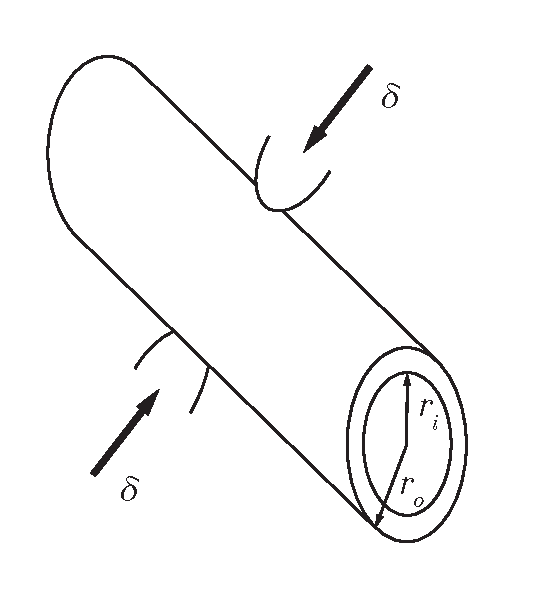
\includegraphics[width=0.5\textwidth]{figuras_3/esquema_arteria.pdf}
\caption{Esquema del problema}
\label{fig:a01}
\end{figure}

Por la configuración de la geometría y las cargas, con el fin de evitarnos sobrecargar el cálculo, decidimos aprovechar la simetría que el problema nos ofrece. Como vemos en la figura \ref{fig:a02}, la geometría diametralmente es simétrica y, además los desplazamientos a imponer, puesto que sera siempre una cantidad $\delta$ a ambos lados, son igualmente simétricos, por lo que solo será necesario modelar 180 grados. Por otro lado, longitudinalmente, podemos coger solo la mitad de la longitud puesto que a ambos lados el desplazamiento es también similar.

\begin{figure}[!htp]
\centering
\begin{subfigure}[b]{0.48\textwidth}
\centering
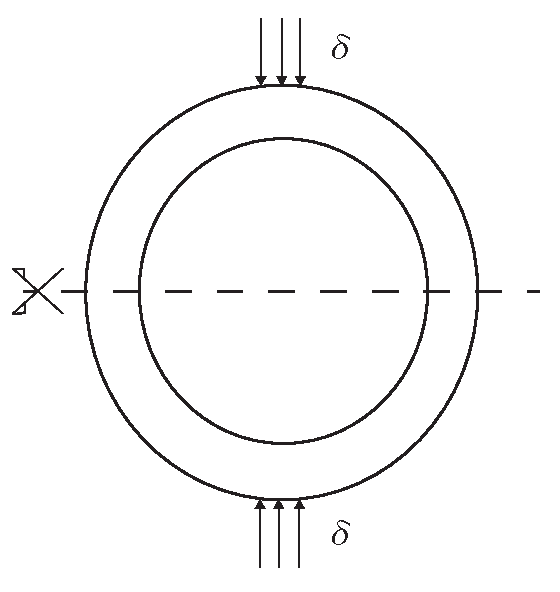
\includegraphics[width=\textwidth]{figuras_3/sim1.pdf}
\caption{Simetría diametral}
\label{fig:a02}
\end{subfigure}
\begin{subfigure}[b]{0.48\textwidth}
\centering
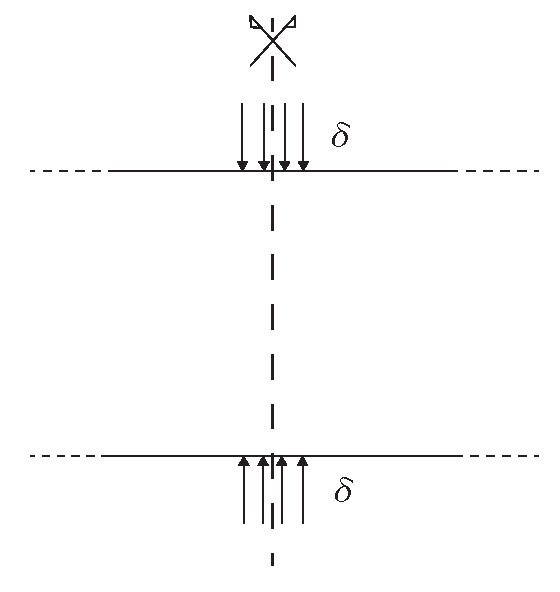
\includegraphics[width=\textwidth]{figuras_3/sim2.pdf}
\caption{Simetría longitudinal}
\label{fig:a03}
\end{subfigure}
\caption{Simetrías que nos ofrece el problema}
\label{fig:a02-03}
\end{figure}

La geometría que dispondremos por tanto será una arteria de 1 mm, radio exterior 1 mm y radio interior 0.9 mm. Solo nos hará falta modelar 180 grados, por lo que el tipo de objeto a elegir será \emph{Solid Arc.} Todos estos datos se muestran en la figura ref{fig:a04}.

\begin{figure}[!htp]
\centering
\includegraphics[width=0.85\textwidth]{figuras_3/a1.png}
\caption{Geometría del problema}
\label{fig:a04}
\end{figure}

En este caso las divisiones de la geometría que impondremos al mallador serán diferentes que las del tipo \emph{Box}: optaremos por 32 divisiones radiales del arco, 4 segmentos por ancho del tubo y 16 divisiones o \emph{Stacks} en el eje longitudinal. Con esto saldrá una malla similar a la de la figura ref{fig:a05}.

\begin{figure}[!htp]
\centering
\includegraphics[width=0.85\textwidth]{figuras_3/a2.png}
\caption{Malla del problema}
\label{fig:a05}
\end{figure}

Para el material tomaremos en primer lugar el modelo Neohookeano, con las mismas propiedades que en la sección anterior (fig \ref{fig:a06}). Hemos de tener en cuenta que hemos llegado a este material con el caso particular de un modelo \emph{Mooney-Rivlin.} Recordar también que en el apartado \emph{Selection}, para que no aparezca ninguna exclamación en nuestro material, debemos tener seleccionada la \emph{parte} donde se encuentre nuestra geometría.

\begin{figure}[!htp]
\centering
\includegraphics[width=0.85\textwidth]{figuras_3/a3.png}
\caption{Material}
\label{fig:a06}
\end{figure}

En cuanto a las condiciones de contorno, han de reflejar las condiciones de simetría mencionadas anteriormente. Por tanto, en el eje radial consideraremos fijar la dirección \emph{y} puesto que es la dirección normal a esa superficie (fig \ref{fig:a07}). Por otro lado, puesto que hay simetría longitudinal y a la vez existe la condición de dominio infinito en el eje longitudinal, podemos también fijar los dos extremos de la arteria que equivalen a los planos \emph{z=0.0} y \emph{z=1.0 }(fig \ref{fig:a08}). Dicha fijación se hace en la dirección normal, la \emph{z.}

\begin{figure}[!htp]
\centering
\begin{subfigure}[b]{0.48\textwidth}
\centering
\includegraphics[width=\textwidth]{figuras_3/a4.png}
\caption{Condición de contorno en \emph{y}}
\label{fig:a07}
\end{subfigure}
\begin{subfigure}[b]{0.48\textwidth}
\centering
\includegraphics[width=\textwidth]{figuras_3/a5.png}
\caption{Condición de contorno en \emph{z}}
\label{fig:a08}
\end{subfigure}
\caption{Condiciones de contorno en desplazamiento igual a 0}
\label{fig:a07-08}
\end{figure}

El desplazamiento impuesto se define como $u_{z}=-1$ mm, aplicado en una zona en la cara superior (habría otra en la cara inferior que no simulamos para reducir el tiempo de computación). Hemos seleccionado 9 nodos cercanos a la superficie $z=1$, en rojo en la figura \ref{fig:a09}, que, o bien se pueden seleccionar uno a uno o seleccionando un nodo de esa zona y activando la opción de adyacentes, con un radio de acción de 2.5. 

\begin{figure}[!htp]
\centering
\includegraphics[width=0.85\textwidth]{figuras_3/a6.png}
\caption{Condición de contorno en desplazamiento impuesto}
\label{fig:a09}
\end{figure}

En este caso tomaremos 20 incrementos, de valor $\Delta t=0.05$, alcanzando un tiempo final de aplicación para la carga $T_\text{fin}=20\times 0.05=1.0$ (fig. \ref{fig:a10}). No se precisa por tanto modificar la curva de carga por defecto que considera un tiempo final $1.0$. Finalmente, se guarda el fichero \texttt{.fsm}, y se realiza el cálculo con FEBiO.

\begin{figure}[!htp]
\centering
\includegraphics[width=0.25\textwidth]{figuras_3/a7.png}
\caption{Condición de cálculo}
\label{fig:a10}
\end{figure}

\subsection{Resultados}

Los resultados en cuanto a mapas de los desplazamientos totales pueden verse en la fig. \ref{fig:a11-12} para las configuraciones sin deformar (t=0) y deformada (t=1). 

\begin{figure}[!htp]
\centering
\begin{subfigure}[b]{0.48\textwidth}
\centering
\includegraphics[width=\textwidth]{figuras_3/a_p1.png}
\caption{Resultados para t=0}
\label{fig:a11}
\end{subfigure}
\begin{subfigure}[b]{0.48\textwidth}
\centering
\includegraphics[width=\textwidth]{figuras_3/a_p2.png}
\caption{resultados para t=1}
\label{fig:a12}
\end{subfigure}
\caption{Mapa de desplazamientos totales}
\label{fig:a11-12}
\end{figure}

Además de otros muchos resultados, nos interesa saber como son las reacciones en la dirección \emph{y}. Para ello vamos a integrar las tensiones en los planos en \textit{y=0.} Para ello, debemos seleccionar el mapa de colores de tensiones en y, $\sigma_{yy}$. A continuación hemos de seleccionar dichos planos. Podemos seleccionar las caras de todos los elementos o, si clickamos en la opción de seleccionar también los adyacentes, seleccionar toda esa superficie de una vez, y pulsando la tecla mayúscula, también añadir la superficie opuesta. Una vez seleccionado pulsamos en el botón \emph{integrate}. Todos estos pasos vienen reflejados en la imagen \ref{fig:a13}. Como vemos, se nos genera una curva que integra las tensiones y que, dividiendo por el área aplicada, nos da una idea de las fuerzas a las que esta sometida esta sección.

\begin{figure}[!htp]
\centering
\begin{subfigure}[b]{0.55\textwidth}
\centering
\includegraphics[width=\textwidth]{figuras_3/a_p3.png}
\caption{Resultados para t=0}
\label{fig:a13}
\end{subfigure}
\begin{subfigure}[b]{0.38\textwidth}
\centering
\includegraphics[width=\textwidth]{figuras_3/a_p4.png}
\caption{resultados para t=1}
\label{fig:a14}
\end{subfigure}
\caption{Mapa de desplazamientos totales}
\label{fig:a13-14}
\end{figure}

\clearpage
\section{Tareas para entregar}
\label{sec:tareas}

Deberán obtenerse y presentarse los siguientes resultados:
\begin{enumerate}
	\item
	Historia de $\sigma_{zz}(t)$ para el modelo homogéneo (1 elemento) Neohookeano, de material de Ogden y otro elástico lineal (buscar parámetros equivalentes sabiendo la equivalencia entre los parámetros del Neo-Hookeano y los modelos volumétrocos y a cortante elásticos) con el fin de comparar los resultados de los diferentes materiales empleados.
	\item
	Para el caso de la arteria, repetir el caso con el material de Ogden y comparar el resultado de la integral de tensiones en \emph{y.} 
	\item
	Se observa en el caso de la arteria (fig~\ref{fig:a12}) como todo el dominio se deforma en la dirección \emph{y}. Sin embargo, el caso esperado sería que solo una pequeña zona se deformase. Con el propósito de buscar este resultado, repetir el cálculo de la arteria con material Neohookeano con una longitud de 4 mm. La malla se hace 4 veces más grande. ¿Qué propondrías para reducir tiempo de cálculo?
\end{enumerate}